\documentclass{beamer}
\beamertemplatenavigationsymbolsempty
\graphicspath {{../../images/}}

\usepackage[utf8]{inputenc}
\usepackage[czech,english]{babel}
\selectlanguage{czech}

\usepackage{amsmath}
\usepackage{amsmath}
\usepackage{tikz}
\usetikzlibrary{arrows.meta, quotes, calc}

\newcommand{\bra}[1]{\langle#1\rvert} % Bra
\newcommand{\ket}[1]{\lvert#1\rangle} % Ket
\newcommand{\qprod}[2]{ \langle #1 | #2 \rangle} %Inner Product
\newcommand{\braopket}[3]{\langle #1 | #2 | #3\rangle} % Matrix Element
\newcommand{\expect}[1]{ \langle #1 \rangle} % Expectation value
\newcommand\abs[1]{\left|#1\right|}



% Theme
\usetheme{Boadilla}

% Title page
\title{Optimalizácia variačných kvantových eigensolverov}
\author{Michal Švec}
\institute{doc. RNDr. Martin Plesch, PhD.}
\date{}

\makeatother
\setbeamertemplate{footline}
{
  \leavevmode%
  \hbox{%
  \begin{beamercolorbox}[wd=.9\paperwidth,ht=2.25ex,dp=1ex,center]{author in head/foot}%
    \usebeamerfont{author in head/foot} Michal Švec \ \ \ \ \ \ \ \ \ \ \ \ \insertshorttitle
  \end{beamercolorbox}%
  \begin{beamercolorbox}[wd=.1\paperwidth,ht=2.25ex,dp=1ex,center]{date in head/foot}%
    \insertframenumber{} /\inserttotalframenumber\hspace*{1ex}
  \end{beamercolorbox}}%
  \vskip0pt%
}
\makeatletter
\setbeamertemplate{navigation symbols}{}
\setbeamertemplate{itemize items}[circle]
\setbeamertemplate{caption}{\raggedright\insertcaption\par}

% Begin document
\begin{document}

% Title slide
\begin{frame}
	\titlepage
\end{frame}

% \begin{frame}
%     \frametitle{Kvantové počítače}
%     \begin{columns}[t]
% 		\begin{column}{.6\textwidth}
% 			\centering	
%             \begin{itemize}
%                 \item riadia sa zákonmi kvantovej mechaniky
%                 \item pravdepodobnostný výpočtový model
%                 \item využitie paralelizmu
%                 \item niektoré problémy dokážu vyriešiť rýchlejšie ako štandardné počítače
%                 \item v súčasnosti ešte nie sú veľmi užitočné, nedokážu vyriešiť nič zmysluplné
%                 \item najväčší problém predstavuje šum a malý počet qubitov
%             \end{itemize}
%         \end{column}
						      
%     \begin{column}{.4\textwidth}
%         \centering                           
%         \begin{figure}
%             \centering
%             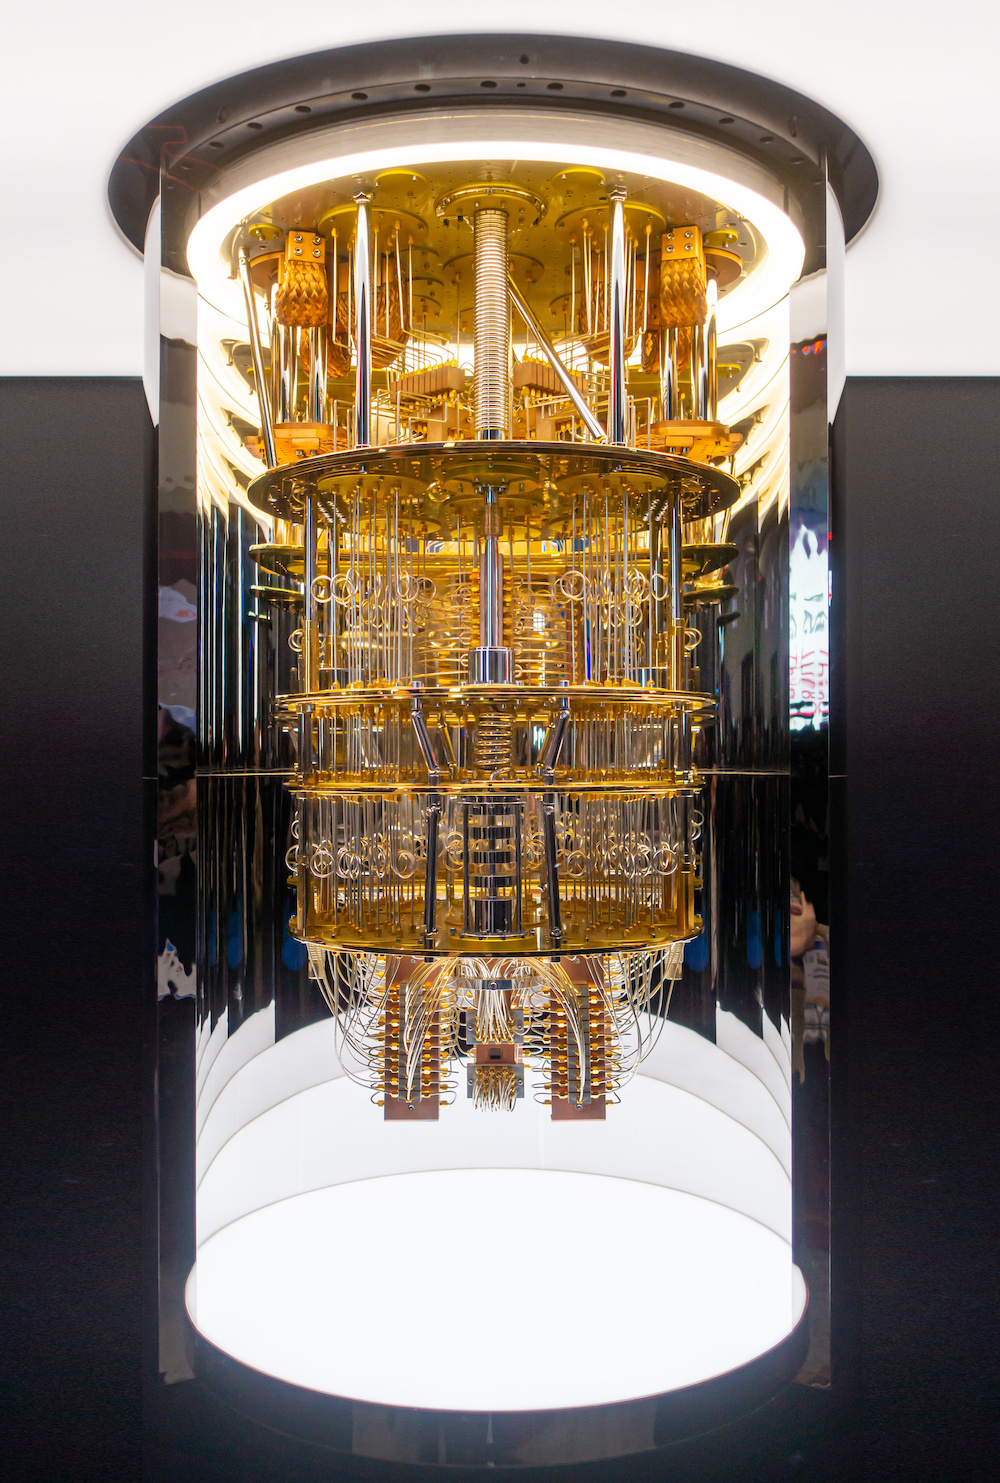
\includegraphics[width=.9\textwidth]{quantum_computer.jpeg}
%             \tiny zdroj:\url{https://theinnovator.news/wp-content/uploads/2023/07/shutterstock_2103465587.jpg}  
                     
%         \end{figure}
%     \end{column}
% \end{columns}

% \end{frame}

\begin{frame}
    \frametitle{Ansatz \& Hamiltonian}
	\begin{itemize}
        \item Ansatz
        \begin{itemize}
            \item parametrizovaný kvantový obvod
            \item zaoberáme sa len triedou hardvérovo efektívnych ansatzov (HEA)
            \begin{itemize}
                \item dajú sa použiť aj na dnešných kvantových počítačoch
                \item sú všeobecné, nie sú viazané na žiadny špecifický problém
            \end{itemize}
        \end{itemize}
        \vspace{10pt}
        % \begin{table}[H]
        %     \renewcommand\arraystretch{1.5}
        %     \centering
        %     \begin{tabular}{|c|c|c|} 
        %         \hline
        %         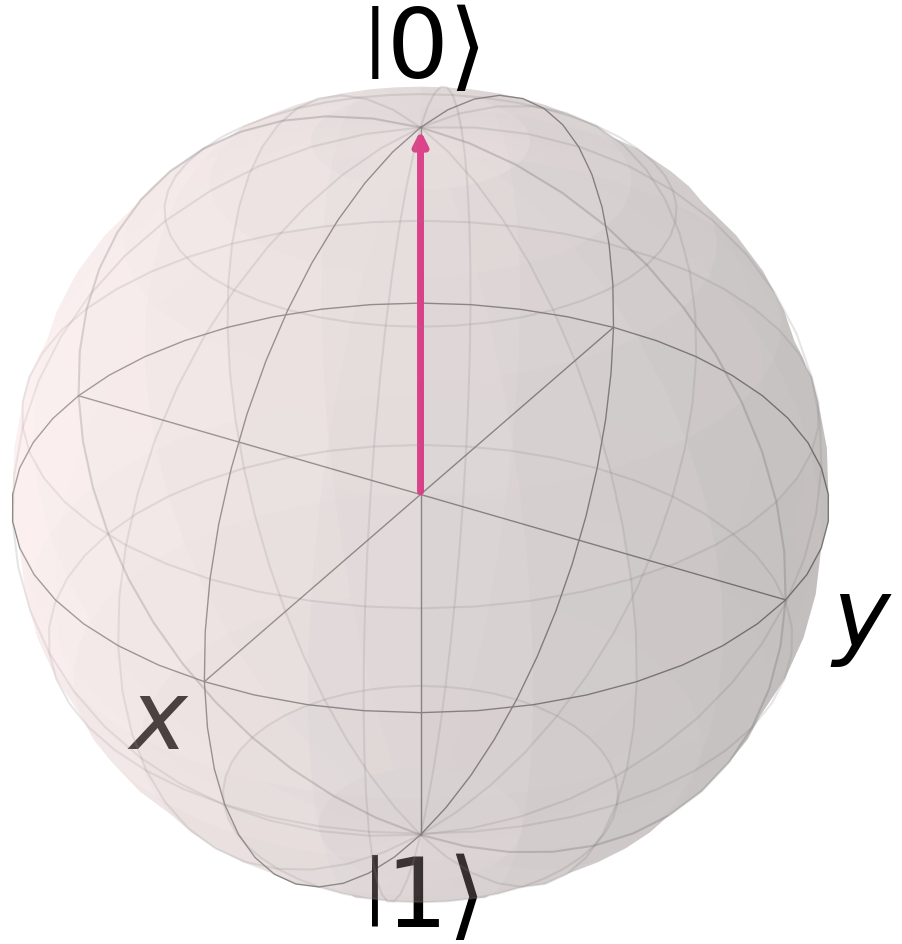
\includegraphics[width=1.5in]{qubit0.png} & 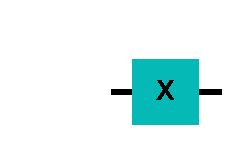
\includegraphics[width=0.6in]{gate-x.pdf}  & \vfill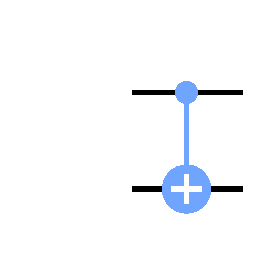
\includegraphics[width=0.6in]{gate-cnot.pdf}\\
        %         Qubit & X hradlo & CNOT hradlo\\
        %         % &&\\[0.5pt]
        %         \hline
        %     \end{tabular}    
        %   \end{table}

        \begin{columns}[c]
            \begin{column}{.4\textwidth}
                \centering
                \begin{figure}
                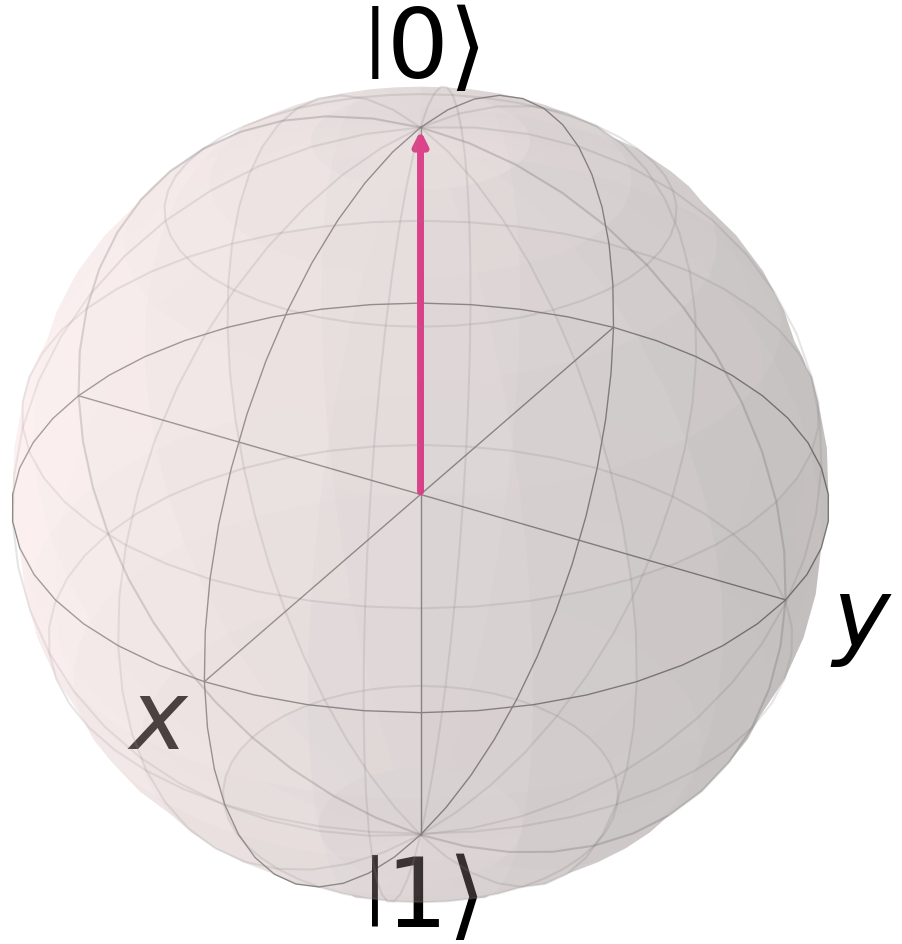
\includegraphics[width=.6\textwidth]{qubit0.png}            
                % \caption{Qubit}
                \end{figure}
            \end{column}
                                  
            \begin{column}{.25\textwidth}
                \centering
                \begin{figure}
                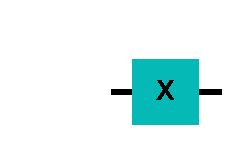
\includegraphics[width=.5\textwidth]{gate-x.pdf}
                \vfill
                % \caption{X hradlo}
                \end{figure}
            \end{column}
            \begin{column}{.25\textwidth}
                \centering
                \begin{figure}
                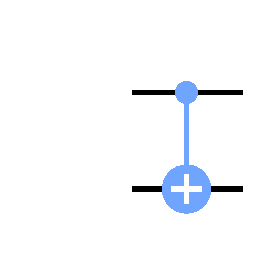
\includegraphics[width=.5\textwidth]{gate-cnot.pdf}
                % \caption{CNOT hradlo}
                \end{figure}

            \end{column}
        \end{columns}
        \item Hamiltonian
        \begin{itemize}
            \item reprezentuje celkovú energiu systému
            \item vybrali sme si molekulu jednu vodíka (H$_2$) reprezentovanú pomocou 4 qubitov
            \item pre nás to je len \textbf{matica} (16 $\times$ 16, máme 4 qubity a $2^4 = 16$)
        \end{itemize}
    \end{itemize}
\end{frame}

\begin{frame}
    \frametitle{Zakladný stav energie}
    \begin{itemize}
        \item stav, kedy sú elektróny najbližšie k jadru
        \item základný stav molekuly vodíka = -1.8671050114542505 Ha
        \item presná hodnota nie je podstatná, sústredíme sa na \textbf{chemickú presnosť} $\pm 0.0016$ Ha
    \end{itemize}
    \centering
    \begin{figure}
        \centering
        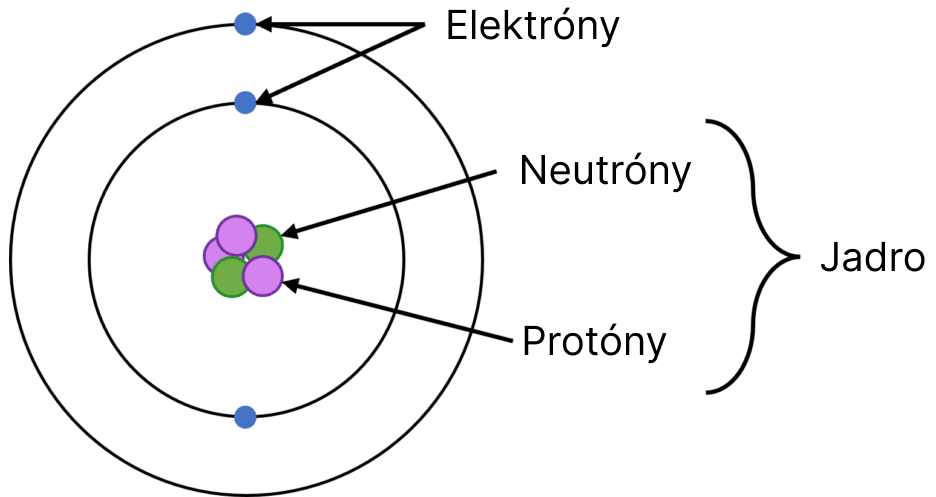
\includegraphics[width=.8\textwidth]{atom-structure-sk.png}
        \tiny zdroj:\url{https://mmerevise.co.uk/app/uploads/2022/10/Atomic-Structure-alevel-1536x779.png.webp}

    \end{figure}
\end{frame}

\begin{frame}
    \frametitle{Variačný kvantový eigensolver (VQE)}
	\begin{itemize}
        \item hybridný algoritmus
        \begin{itemize}
            \item časť práce odovzdáme klasickému počítaču
            \item na klasickom počítači beží optimalizačný algoritmus
        \end{itemize}
    \end{itemize}
    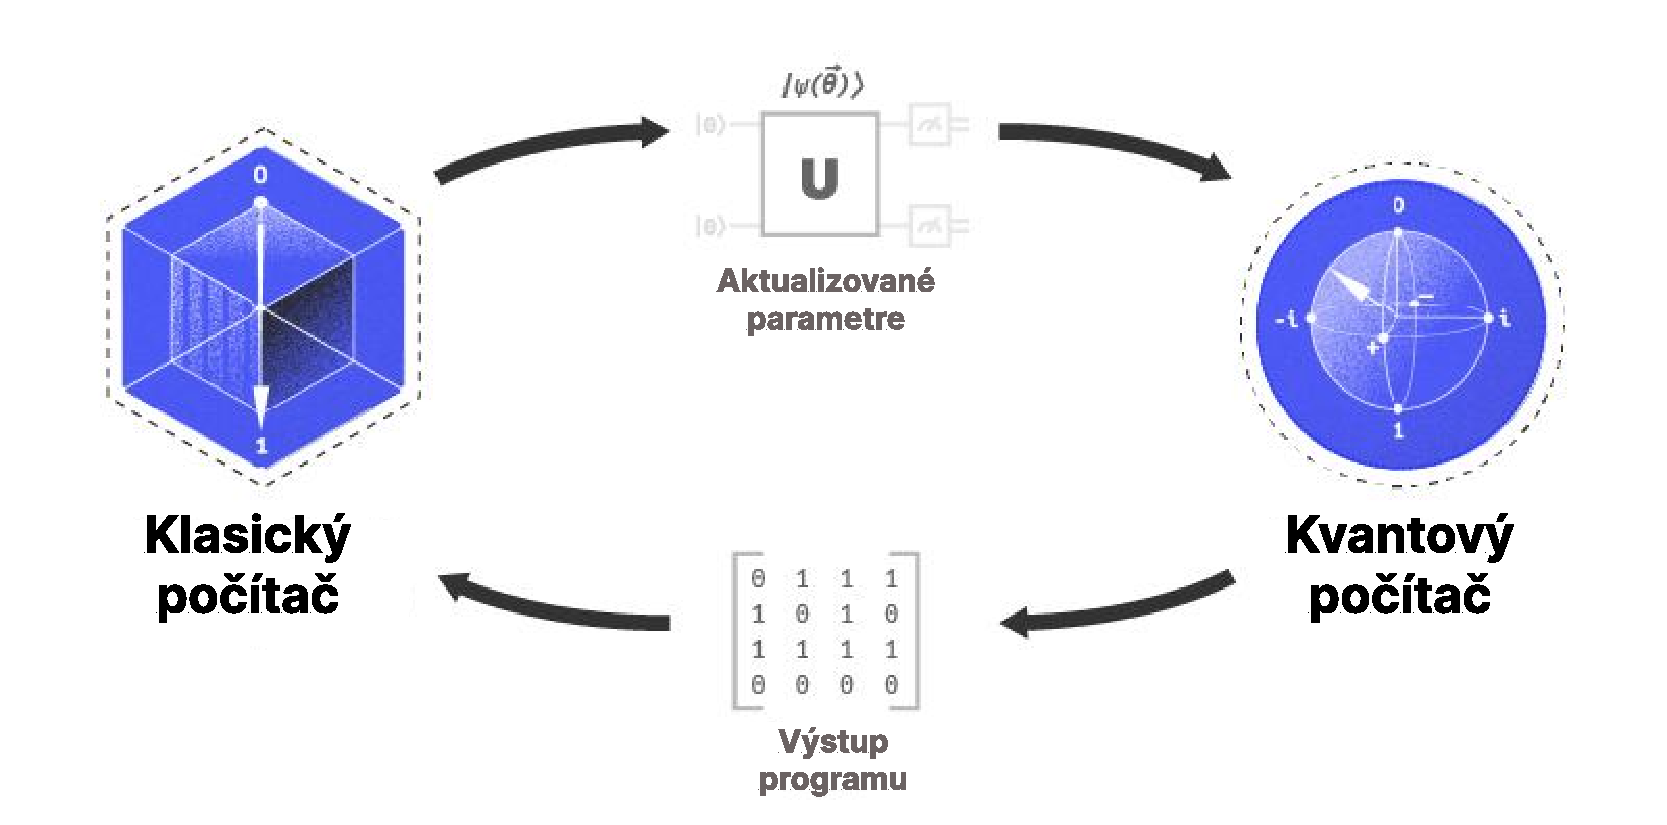
\includegraphics[width=1\textwidth]{vqe-hybrid-sk.pdf}
    \tiny zdroj:\url{https://images.ctfassets.net/hqm865gc1xfs/7ADhfqvgYOEesM5oSFHCiL/eb70f8716e2831015253e1eedced6320/2022-01-06-vqe.jpeg}  
    
    % \begin{itemize}
    %     \item kvantový počítač sa strieda s kvantovým
    %     \begin{itemize}
    %         \item zastaví sa po dosiahnutí určitého stanoveného počtu iterácií alebo po nájdení výsledku
    %     \end{itemize}
    % \end{itemize}
\end{frame}

\begin{frame}
    \frametitle{Variačný kvantový eigensolver (VQE)}
    \begin{itemize}
        \item rôzne možnosti použitia
        \item zaoberáme sa nájdením základného stavu molekuly vodíka
        % \item variačná metóda
        % \begin{itemize}
        %     \item umožňuje nájsť aproximáciu základného stavu
        % \end{itemize}
        \item eigensolver
        \begin{itemize}
            \item nájde najmenšie vlastné číslo = základný stav 
        \end{itemize} 
        \item cieľovú funkciu tvorí ansatz a Hamiltonian
    \end{itemize}
    \begin{columns}[T] % align columns at the top
        \begin{column}{0.0\textwidth} % adjust the left margin
        \end{column}
        \begin{column}{0.95\textwidth} % adjust the width of the block
            \begin{tikzpicture}
                \node[draw, rectangle, minimum width = 1.5 cm, minimum height = 1.5 cm] (fl) at (0,0) {VQE};
                \node[above] at (fl.north) {};
                \draw [Triangle-] (fl.west) -- node[above]{Hamiltonian} node[below]{ansatz} ++(-5.5,0);
                \draw [-Triangle] (fl.east) -- node[above]{základný stav energie} node[below]{} ++(4,0);
            \end{tikzpicture}
        \end{column}
    \end{columns}
    \begin{block}{Cieľ}
        \begin{itemize}
            \item zamerali sme sa na výkonnosť VQE
            \item zisťovali sme, ako jednotlivé ansatze a optimalizačné algoritmy ovplyvňujú výsledok
        \end{itemize}
    \end{block}
\end{frame}

\begin{frame}
    \frametitle{Linear ansatz}
	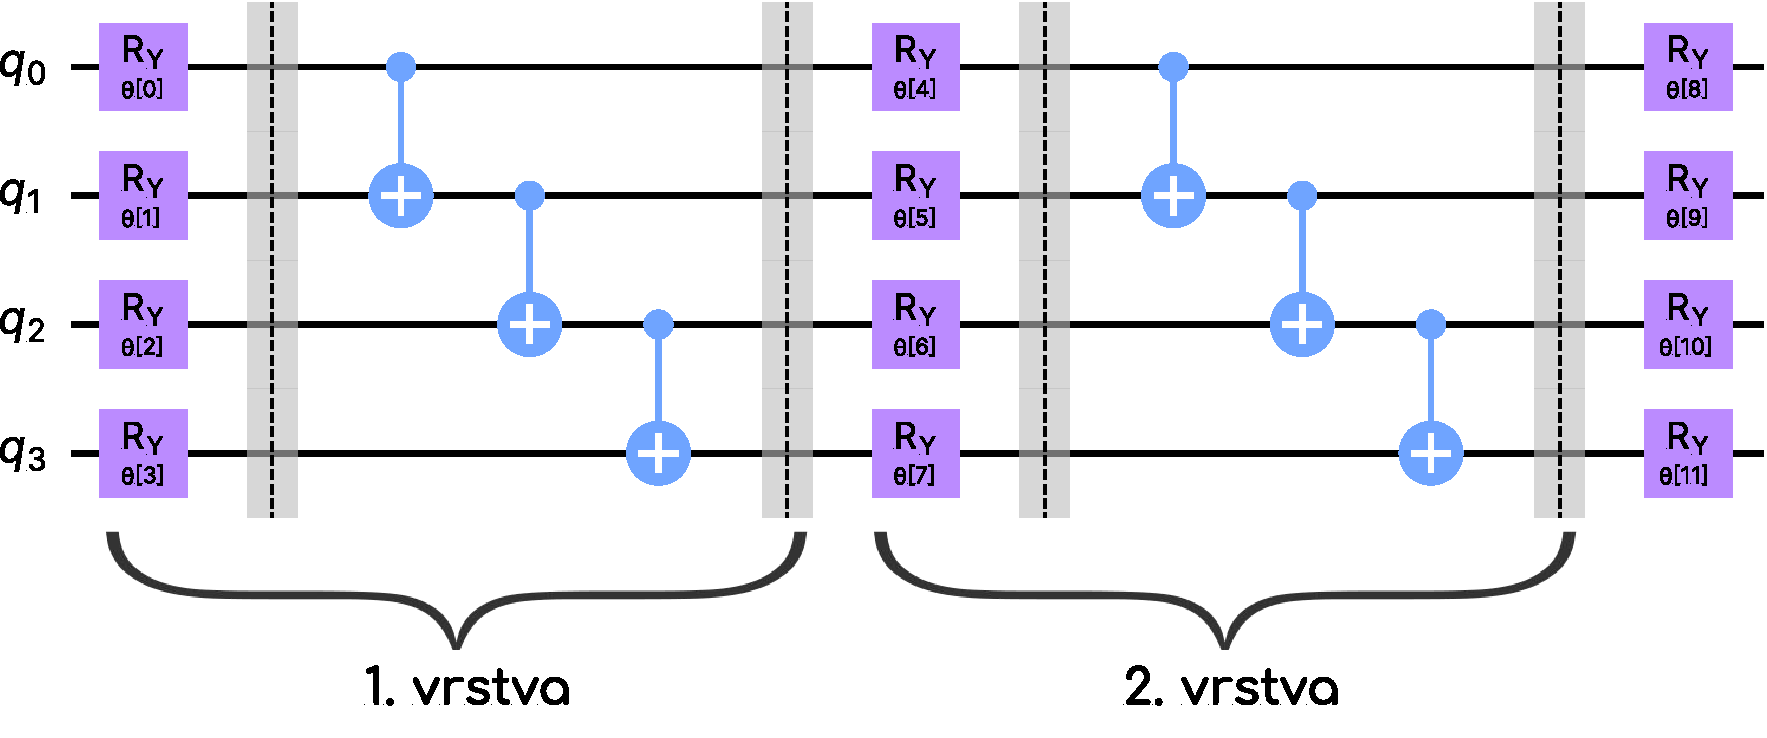
\includegraphics[width=1\textwidth]{anstaz-linear-layers.pdf}
    \begin{itemize}
        \item vrstva sa skladá z rotačných hradiel a previazania
        \item každý qubit je previazaný s nasledujúcim
    \end{itemize}
\end{frame}

\begin{frame}
    \frametitle{Reverse linear ansatz}
	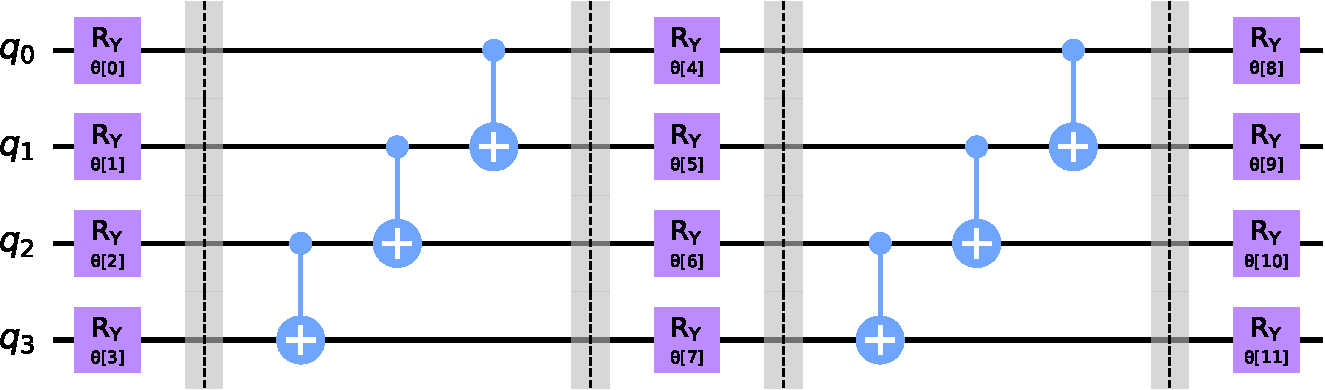
\includegraphics[width=1\textwidth]{ansatz-reverse-linear.pdf}
    \begin{itemize}
        \item taký istý ako linear ansatz, ale qubity sú previazané v opačnom poradí
    \end{itemize}
\end{frame}

% \begin{frame}
%     \frametitle{Pairwise ansatz}
% 	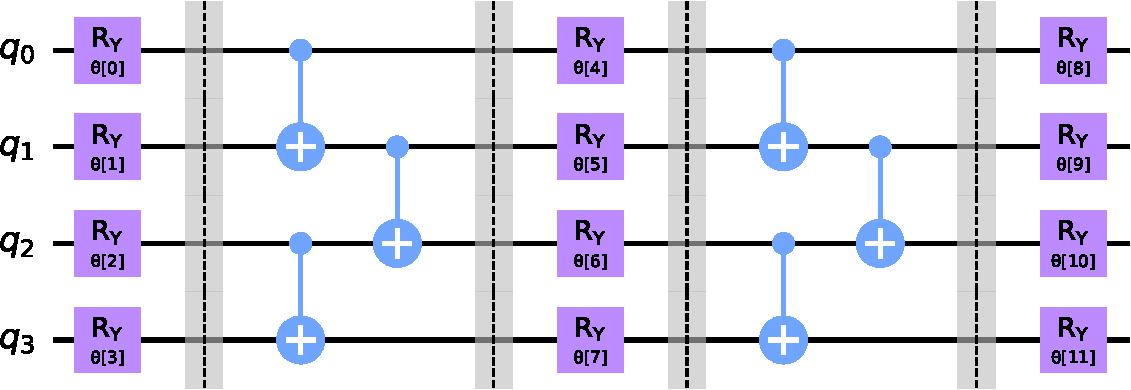
\includegraphics[width=1\textwidth]{ansatz-pairwise.pdf}
%     \begin{itemize}
%         \item previazanie je v dvoch úrovniach
%         \begin{itemize}
%             \item na prvej úrovni je qubit $i$ previazaný s qubitom $i + 1$ pre všetky párne $i$ \item na druhej úrovni je qubit $i$ previazaný s qubitom $i + 1$ pre všetky nepárne $i$ 
%         \end{itemize}
%     \end{itemize}
% \end{frame}

\begin{frame}
    \frametitle{Circular ansatz}
	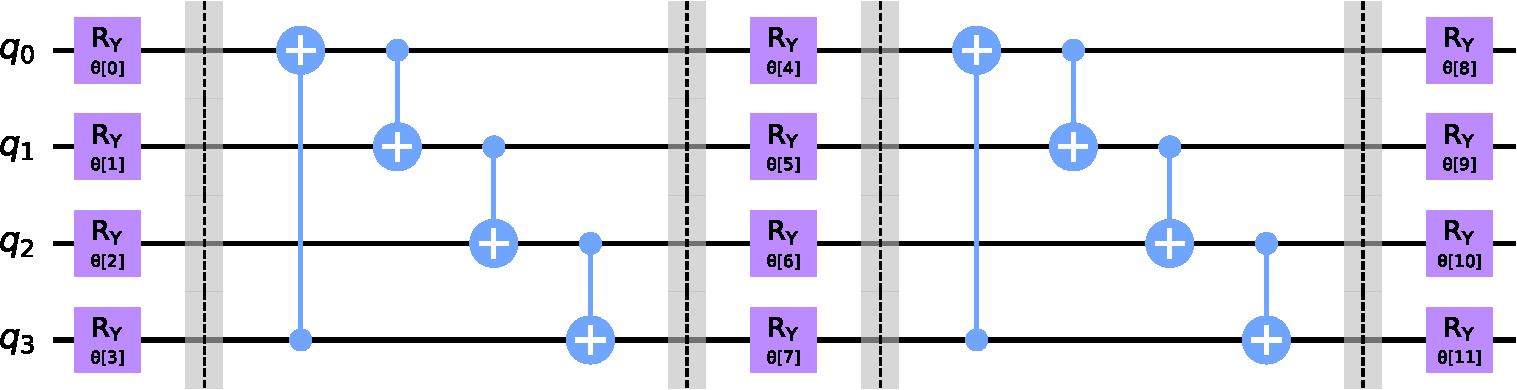
\includegraphics[width=1\textwidth]{ansatz-circular.pdf}
    \begin{itemize}
        \item linear ansatz, ale navyše je posledný qubit previazaný s prvým
    \end{itemize}
\end{frame}

% \begin{frame}
%     \frametitle{Shifted circular alternating (SCA) ansatz}
% 	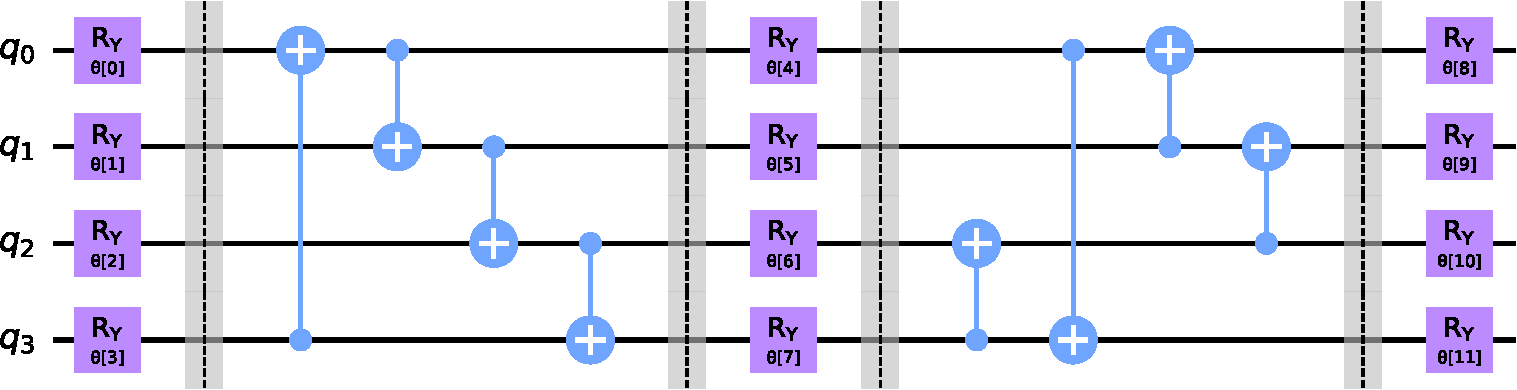
\includegraphics[width=1\textwidth]{ansatz-sca.pdf}
%     \begin{itemize}
%         \item pozostáva z circular ansatzu, ale CNOT, ktorý spája prvý qubit s posledným je posunutý o jedno miesto doprava v každej vrstve
%         \item okrem toho sa v každej vrstve striedajú úlohy zdrojového a cieľového qubitu (alternating)
%     \end{itemize}
% \end{frame}

\begin{frame}
    \frametitle{Full ansatz}
	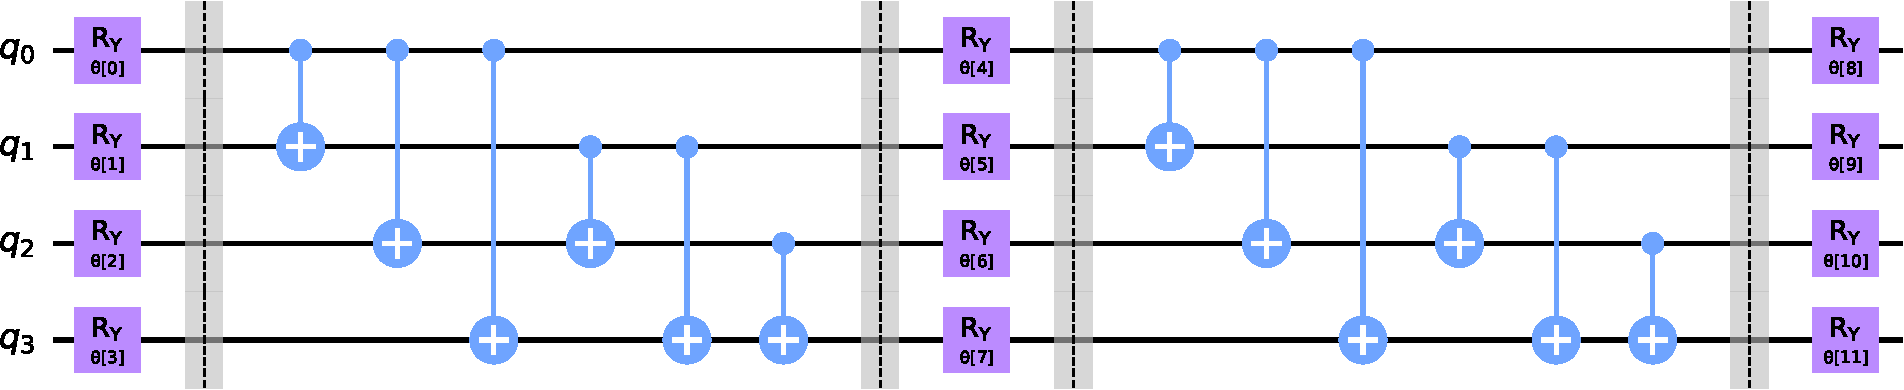
\includegraphics[width=1\textwidth]{ansatz-full.pdf}
    \begin{itemize}
        \item každý qubit je previazaný s každým
    \end{itemize}
\end{frame}

% \begin{frame}
%     \frametitle{Príklad konvergencie energie dvoch optimalizačných algoritmov}
% 	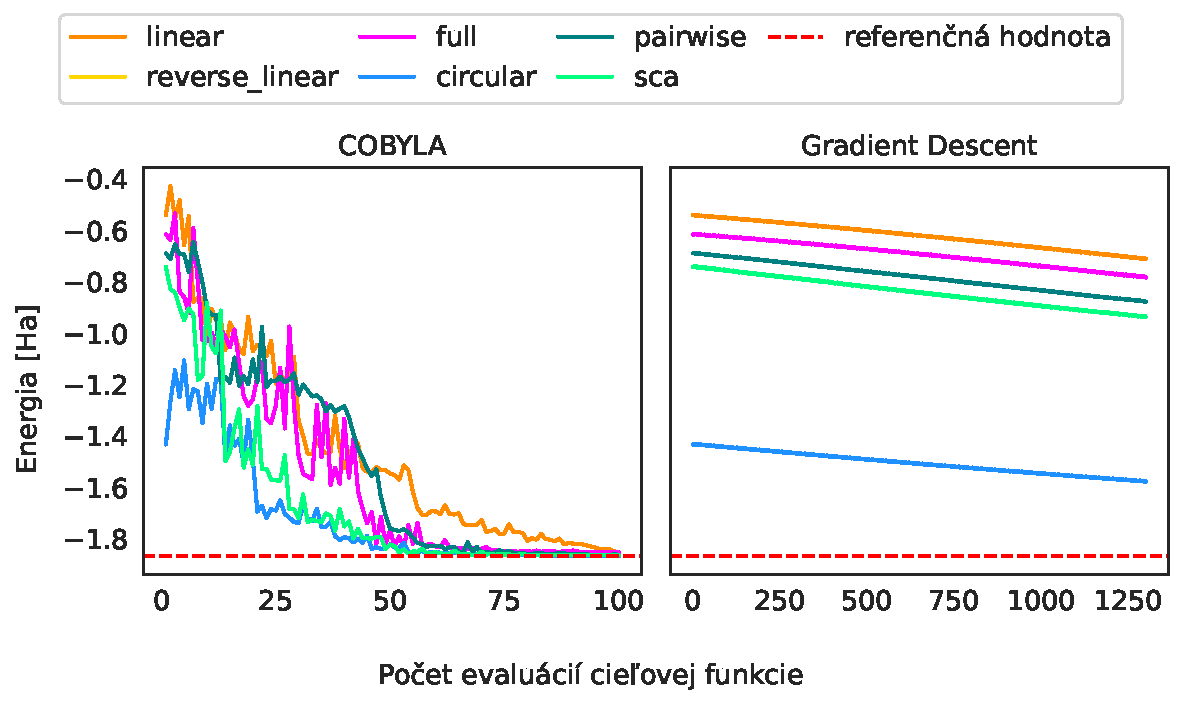
\includegraphics[width=1\textwidth]{convergence_example-sk.pdf}
% \end{frame}

\begin{frame}
    \frametitle{Porovnávanie výkonnosti VQE}
	\begin{itemize}
        \item porovnávali sme, ako jednotlivé kvantové obvody fungujú spolu s optimalizačnými algoritmami
        \item \textbf{15} optimalizačných algoritmov
        \begin{itemize}
            \item v našom prípade optimalizujú parametre pre rotačné hradla ansatzu
            \item algoritmy majú veľa parametrov
            \item zvolili predvolené parametre
            \item nastavili sme len maximum iterácií na \textbf{100}
        \end{itemize}
    \end{itemize}
          
        \begin{table}[H]
            \centering
            \begin{tabular}{|l|c|c|} 
                \hline
                \multicolumn{2}{|c|}{\textbf{Optimalizačné algoritmy}}\\
                \hline
                \multicolumn{1}{|c|}{\textbf{negradientové}} & \textbf{gradientové}\\
                \hline
                AQGD & Gradient Descent \\ 
                \hline
                NFT & CG \\ 
                \hline
                QNSPSA & ADAM \\ 
                \hline
                SPSA & AMSGRAD \\ 
                \hline
                COBYLA & L\_BFGS\_B \\ 
                \hline
                Nelder Mead & SLSQP \\ 
                \hline
                Powell & TNC \\ 
                \hline
                UMDA &  \\
                \hline
            \end{tabular}
        \end{table}

\end{frame}

\begin{frame}
    \frametitle{Porovnávanie výkonnosti VQE}
	\begin{itemize}
        \item \textbf{18} rôznych ansatzov
        \begin{itemize}
            \item 6 typov
            \item z každého typu sme zobrali 1, 2 a 3 vrstvové varianty
        \end{itemize} 
        \item každú kombináciu ansatzu a optimalizačného algoritmu sme spustili 50-krát
        \item vyprodukovali sme dáta a následne sme ich analyzovali
    \end{itemize}
		
            \begin{table}[H]
                \centering
                \begin{tabular}{|l|c|c|} 
                    \hline
                    \multicolumn{1}{|c|}{\textbf{Ansatze}}\\
                    \hline
                    linear \\ 
                    \hline
                    reverse linear \\ 
                    \hline
                    pairwise \\ 
                    \hline
                    circular \\ 
                    \hline
                    SCA \\ 
                    \hline
                    full \\ 
                    \hline
                \end{tabular}
            \end{table}
\end{frame}

\begin{frame}
    \frametitle{Implementácia}
    \begin{itemize}
        \item Qiskit (Quantum Information Science Kit)
        \begin{itemize}
        \item knižnica na prácu s kvantovými počítačmi a kvantovými algoritmami
        \item simulátor
        \item ideálne podmienky, žiadny šum a rušenie 
        \item Python
        \item multiprocessing
        \end{itemize}
    \end{itemize}
    \begin{itemize}
        \item analýza dát
        \begin{itemize}
            \item veľa dát
            \item celkovo 13500 behov VQE
            \begin{itemize}
                \item 15 optimalizačných algoritmov $\times$ 18 ansatzov $\times$ 50-krát
            \end{itemize}
            \item hľadali sme rôzne súvislosti a vhodnú reprezentáciu výsledkov
            \item používali sme knižnice ako Pandas, Plotly, Matplotlib, Seaborn 
        \end{itemize}
    \end{itemize}
\end{frame}

\begin{frame}
    \frametitle{Vplyv vrstiev ansatzu} 
	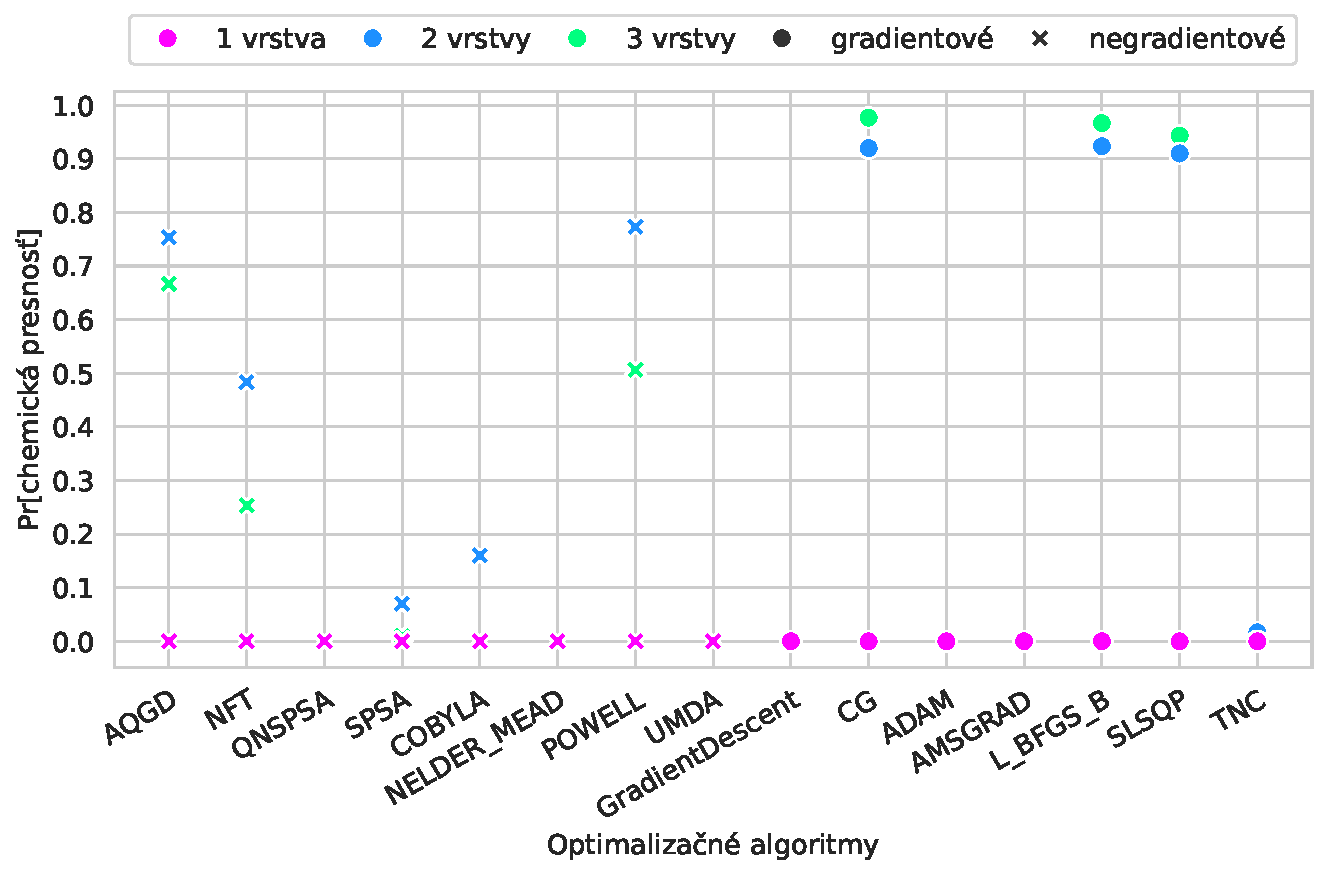
\includegraphics[width=1\textwidth]{layers-sk.pdf}
\end{frame}

\begin{frame}
    \frametitle{Výkonnosť rôznych typov ansatzov}
	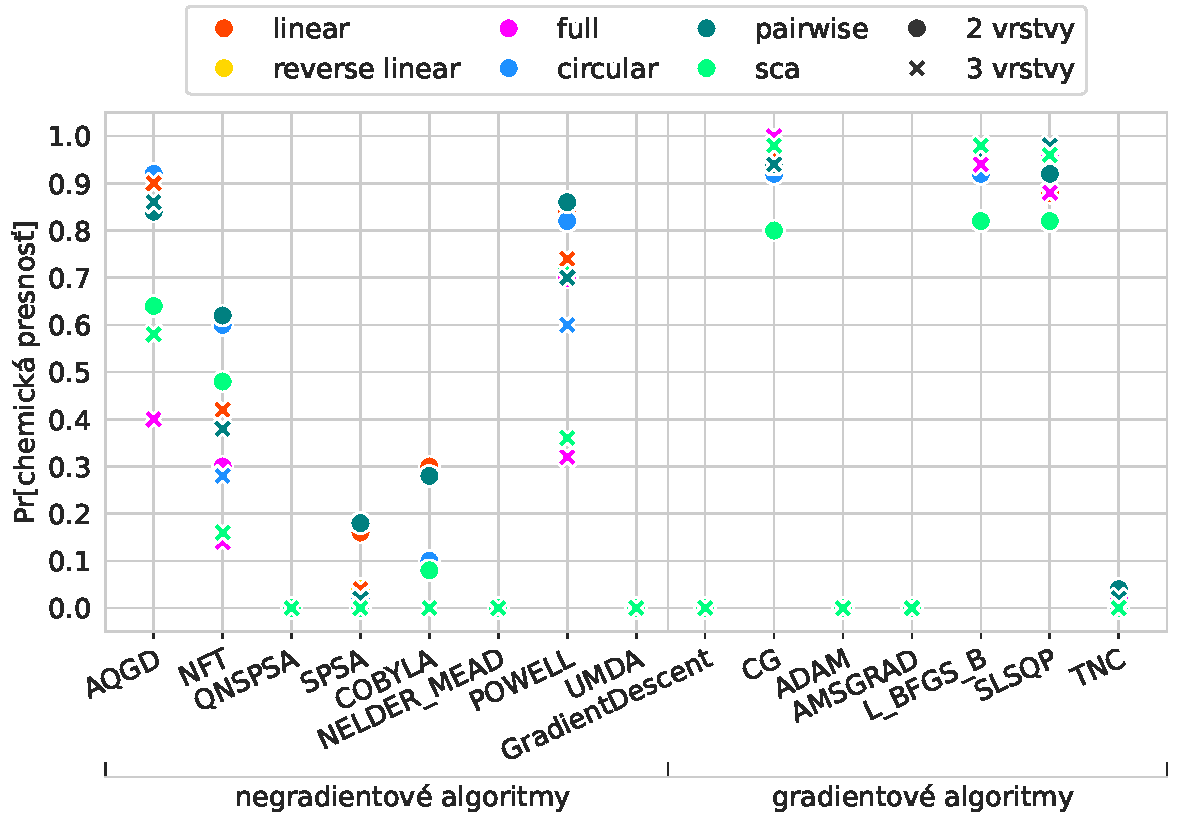
\includegraphics[width=1\textwidth]{chemical-sk.pdf}
\end{frame}

\begin{frame}
    \frametitle{Počet evaluácií cieľovej funkcie \& chemická presnosť} 
	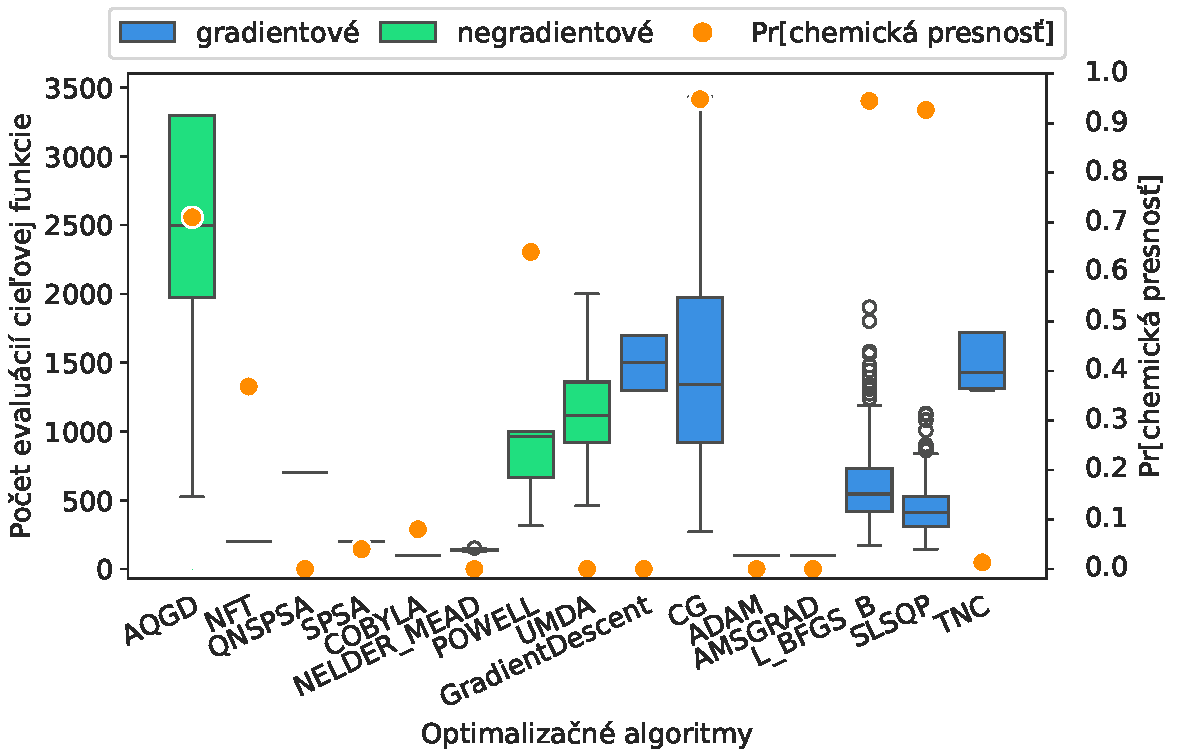
\includegraphics[width=1\textwidth]{evaluations-sk.pdf}
\end{frame}

\begin{frame}
    \frametitle{Priemerný počet dosiahnutí chemickej presnosti za hodinu}
	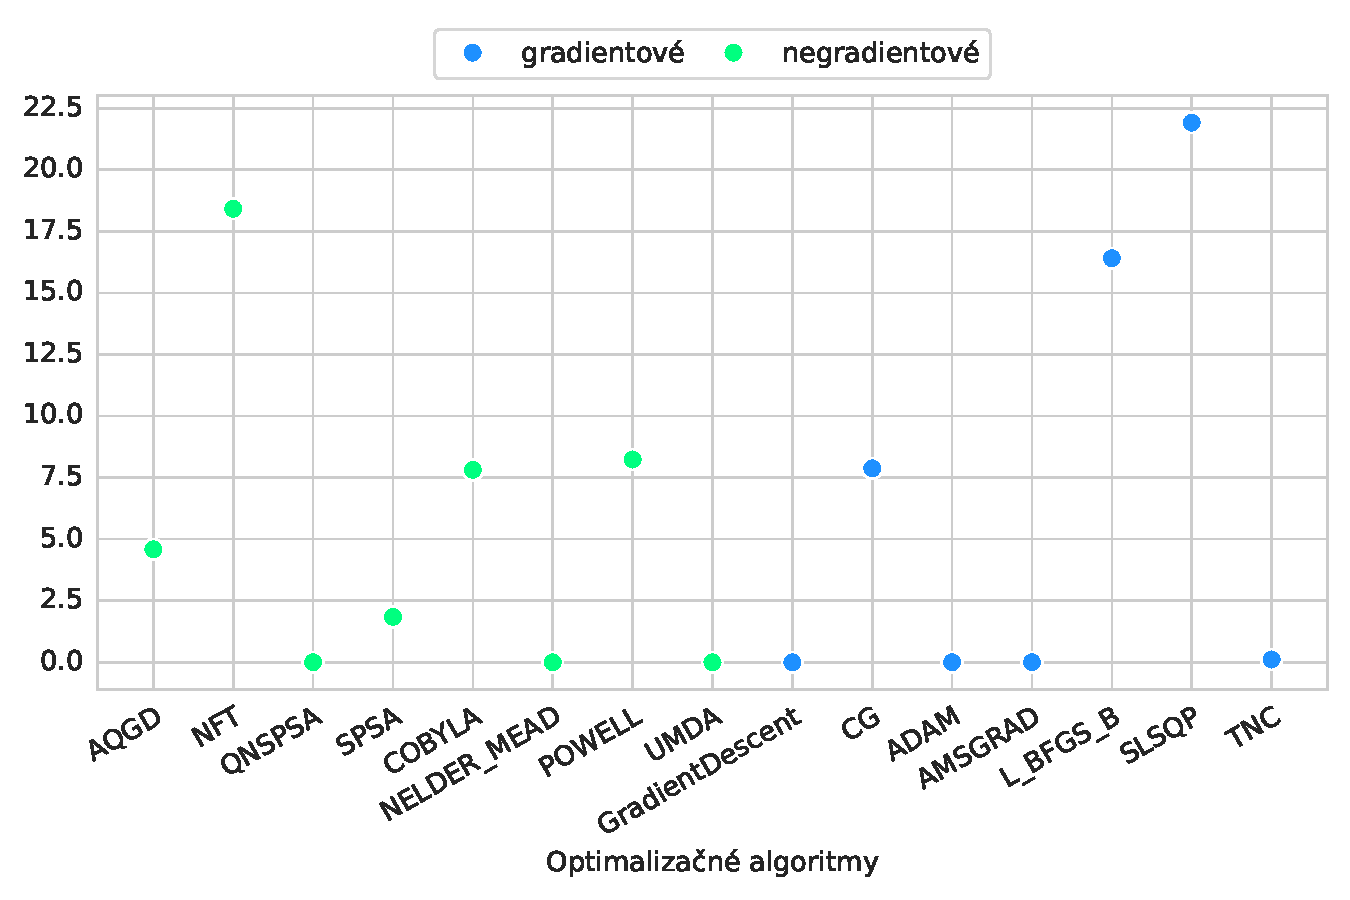
\includegraphics[width=1\textwidth]{hours-sk.pdf}
\end{frame}

\begin{frame}
    \frametitle{Zhrnutie}
    \begin{block}{Ansatze}
        \begin{itemize}
            \item akýkoľvek ansatz s jednou vrstvou nevedie k riešeniu
            \item pri gradientových algoritmoch na voľbe ansatzu až tak nezáleží
            \item negradientové algoritmy sú citlivejšie na voľbu ansatzu
        \end{itemize}
    \end{block}

    \begin{block}{Optimalizačné algoritmy}
        \begin{itemize}
            \item gradientové fungujú lepšie pre ansatze s troma vrstvami
            \item negradientové dosahujú lepšie výsledky s ansatzmi, ktoré majú dve vrstvy
            \item voľba optimalizačného algoritmu je dôležitejšia ako voľba ansatzu
        \end{itemize}
    \end{block}
	
\end{frame}

\end{document}